\documentclass[final,hyperref={pdfpagelabels=false}]{beamer}
\usepackage{grffile}
\mode<presentation>{\usetheme{I6pd2}}
\usepackage[english]{babel}
\usepackage[latin1]{inputenc}
\usepackage{amsmath,amsthm, amssymb, latexsym}
%\usepackage{times}\usefonttheme{professionalfonts}  % obsolete
%\usefonttheme[onlymath]{serif}
\boldmath
\usepackage[orientation=landscape,size=a0,scale=1.4,debug]{beamerposter}
% change list indention level
% \setdefaultleftmargin{3em}{}{}{}{}{}


%\usepackage{snapshot} % will write a .dep file with all dependencies, allows for easy bundling

\usepackage{array,booktabs,tabularx}
\newcolumntype{Z}{>{\centering\arraybackslash}X} % centered tabularx columns
\newcommand{\pphantom}{\textcolor{ta3aluminium}} % phantom introduces a vertical space in p formatted table columns??!!

\listfiles

%%%%%%%%%%%%%%%%%%%%%%%%%%%%%%%%%%%%%%%%%%%%%%%%%%%%%%%%%%%%%%%%%%%%%%%%%%%%%%%%%%%%%%
\graphicspath{{figures/}}

\title{\huge Geo-Language Games: An Agent-Based Model of the Role of Terrain in Language Diversity}
\author{Rachel Hendery, Liam Magee}
\institute[University of Western Sydney]{Digital Humanities Research Group, University of Western Sydney, Parramatta, Australia}
\date[Jun. 29, 2015]{Jun. 29, 2015}

%%%%%%%%%%%%%%%%%%%%%%%%%%%%%%%%%%%%%%%%%%%%%%%%%%%%%%%%%%%%%%%%%%%%%%%%%%%%%%%%%%%%%%
\newlength{\columnheight}
\setlength{\columnheight}{65cm}

% \usepackage{graphicx}
% \usepackage{epstopdf}
% \DeclareGraphicsExtensions{.eps, .png}

%%%%%%%%%%%%%%%%%%%%%%%%%%%%%%%%%%%%%%%%%%%%%%%%%%%%%%%%%%%%%%%%%%%%%%%%%%%%%%%%%%%%%%
\begin{document}
\begin{frame}
  \begin{columns}
    % ---------------------------------------------------------%
    % Set up a column
    \begin{column}{.33\textwidth}
      \begin{beamercolorbox}[center,wd=\textwidth]{postercolumn}
        \begin{minipage}[T]{.95\textwidth}  % tweaks the width, makes a new \textwidth
          \parbox[t][\columnheight]{\textwidth}{ % must be some better way to set the the height, width and textwidth simultaneously
            % Since all columns are the same length, it is all nice and tidy.  You have to get the height empirically
            % ---------------------------------------------------------%
            % fill each column with content
            \begin{block}{Introduction}
              \begin{itemize}
              \item Origins of linguistic diversity are a matter of much debate
              \item For example, PNG has:
                \begin{itemize}
                \item 0.1\% of the world's population
                \item 13\% of the world's languages
                \end{itemize}
              \item Many factors have been proposed to account for diversity (e.g. Pawley 2007; Currie \& Mace 2009; Lupyan \& Dale 2010; Greenhill 2014)
              \item It has been suggested terrain may play a role (e.g. Marck 1986, 2000), but this is rarely included in modern models
              \item Here we:
              \begin{itemize}
            \item argue that GIS \& ABMs offer useful ways to understand role of geography as well as other factors in language change
              \item compare \textit{NetLogo} to custom WebGL 3D visualisations \end{itemize}
              \end{itemize}
            \end{block}
            \vfill
            \begin{block}{General Model}
              \begin{columns}
                \begin{column}{.99\textwidth}
                  \begin{itemize}
                    \item Agents are:
                      \begin{itemize}
                        \item Motile: semi-random movement, constrained by preference for like terrain (limited movement up or down)
                        \item Linguistic: agents have a constrained lexicon of 10 items
                        \item Influential: agents can vary their lexicon under influence of neighbouring agents
                        \item Transmissive: agents pass on lexicographic information to their offspring
                      \end{itemize}
                    \item Simulation includes:
                      \begin{itemize}
                        \item Sample terrain, including a valley and hillside
                        \item Two notional language variants (agents' lexicons can feature items from both)
                        \item Scalar parameters for:
                          \begin{itemize}
                            \item Initial language balance
                            \item Rate of influence
                            \item Rate of emigration
                            \item Transmissive mode - both or a single parent
                          \end{itemize}
                      \end{itemize}
                  \end{itemize}
                \end{column}
              \end{columns}
            \end{block}
            \vfill
            \begin{block}{Model Running in \textit{NetLogo}}
              \begin{figure}
                \centering
                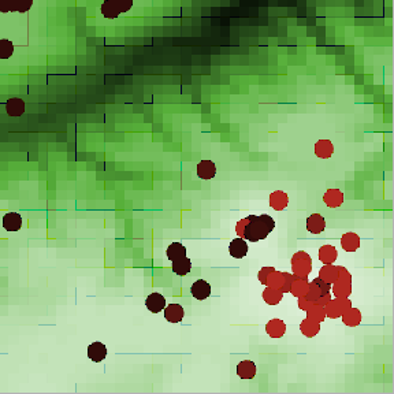
\includegraphics[width=0.32\linewidth]{images/netlogo}
                -
                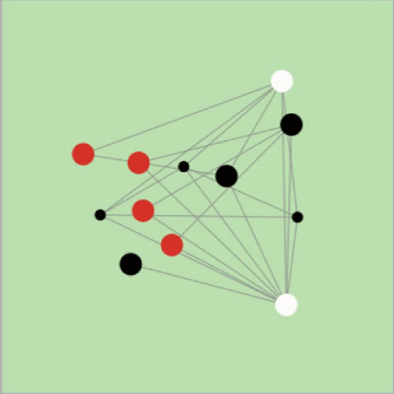
\includegraphics[width=0.32\linewidth]{images/networks}
                -
                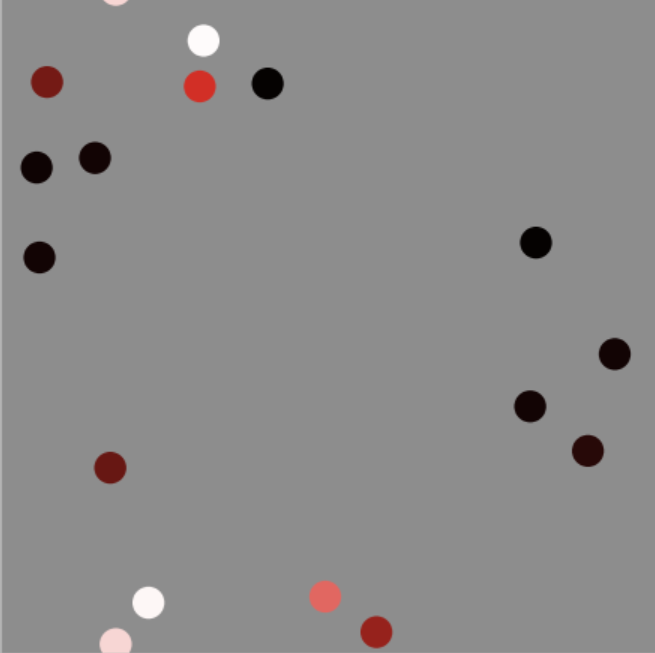
\includegraphics[width=0.32\linewidth]{images/random_movement}
              \end{figure}
            \end{block}
          }
        \end{minipage}
      \end{beamercolorbox}
    \end{column}
    % ---------------------------------------------------------%
    % end the column

    % ---------------------------------------------------------%
    % Set up a column
    \begin{column}{.33\textwidth}
      \begin{beamercolorbox}[center,wd=\textwidth]{postercolumn}
        \begin{minipage}[T]{.95\textwidth} % tweaks the width, makes a new \textwidth
          \parbox[t][\columnheight]{\textwidth}{ % must be some better way to set the the height, width and textwidth simultaneously
            % Since all columns are the same length, it is all nice and tidy.  You have to get the height empirically
            % ---------------------------------------------------------%
            % fill each column with content

            \begin{block}{Language Change}
              \begin{columns}
                \begin{column}{.99\textwidth}
                  \begin{figure}
                    \centering
                    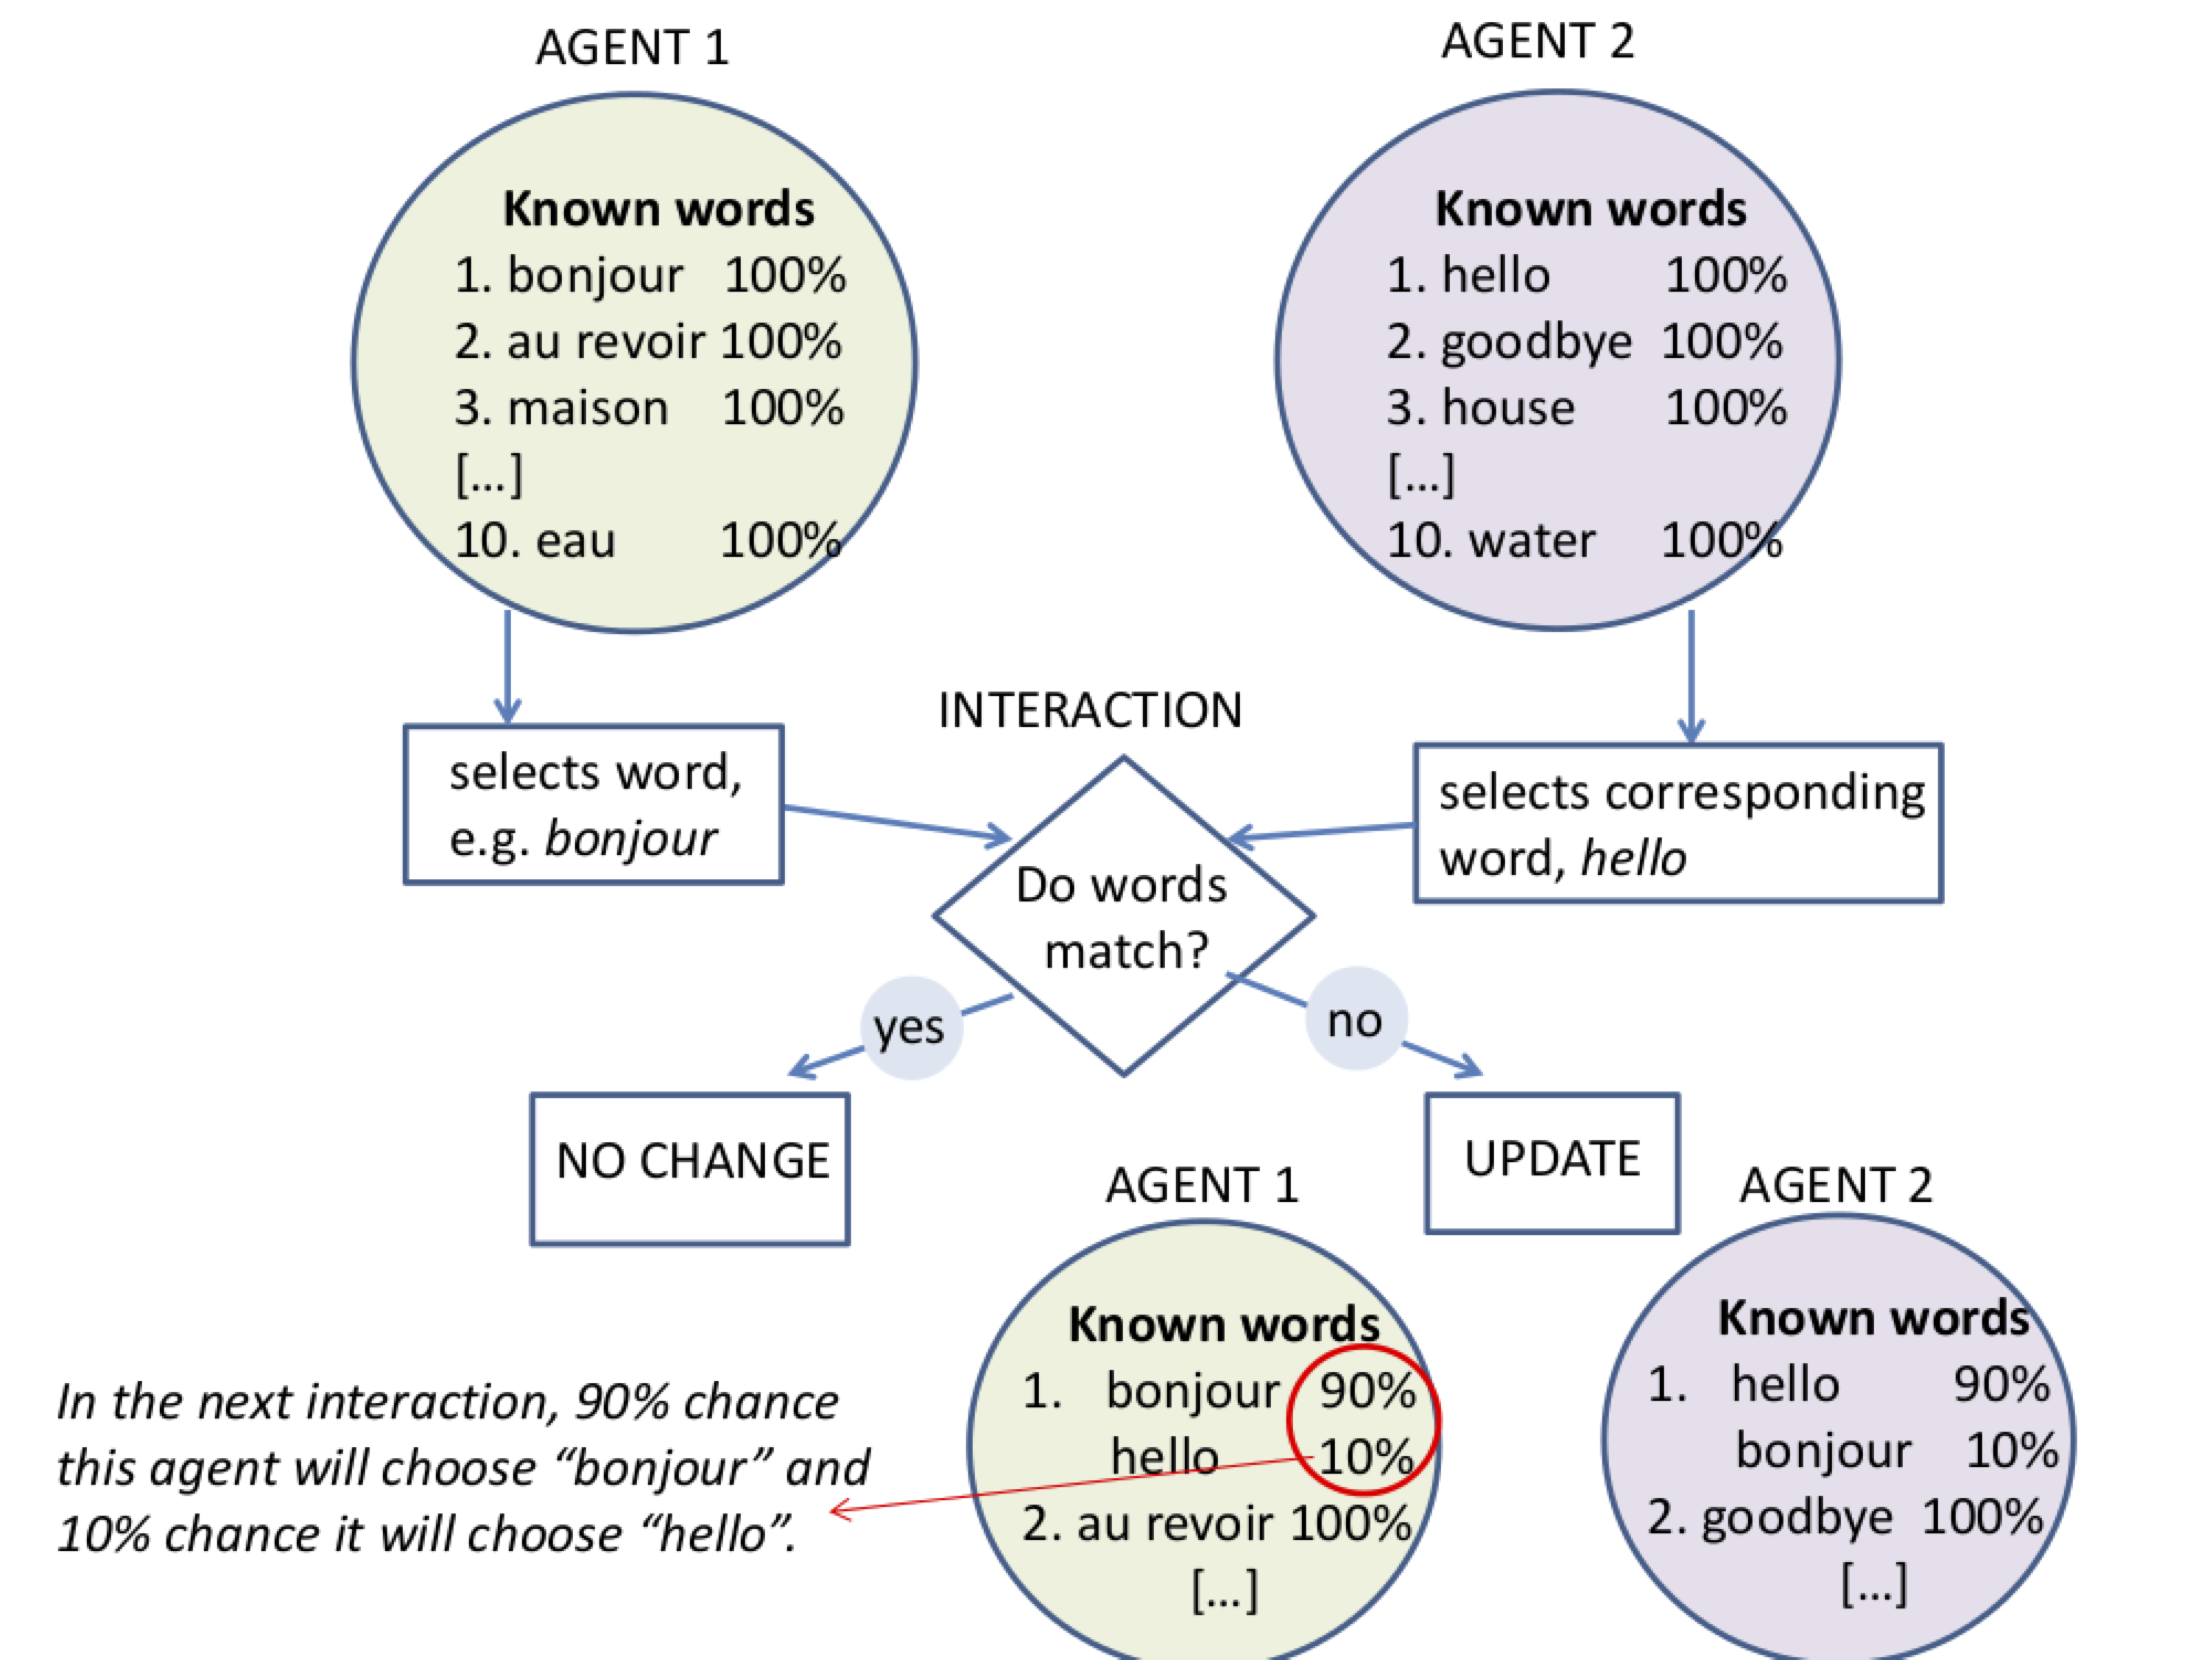
\includegraphics[width=0.80\linewidth]{images/language_change_model}
                  \end{figure}
                  \begin{itemize}
                    \item ANY TEXT NEEDED HERE?
                  \end{itemize}
                \end{column}
              \end{columns}
            \end{block}
            \vfill
            \begin{block}{Descriptive Results}
              \begin{columns}
                \begin{column}{.99\textwidth}
                  \begin{itemize}
                    \item With sufficiently low or high initial language imbalance, one language comes to dominate
                    \item At language balance at close to 50\%, linguistic diversity is retained
                    \item Dialects with a mixed-origin lexicon can develop in hard-to-reach locations with heterogenous initial populations
                    \item "Ethnocentrism"-type (Axelrod \& Hammond 2003) clustering patterns emerge, partially shaped by topography
                    \item Suggests higher "cost" of movement (e.g. here to higher or lower rather than same elevation) is a plausible deterrent to
                     contact-induced language change
                      \begin{itemize}
                        \item Irregular topography can help explain preservation of linguistic diversity, even in relatively dense geographies
                      \end{itemize}
                  \end{itemize}
                \end{column}
              \end{columns}
            \end{block}
            \vfill
            \begin{block}{Further Refinements}
              \begin{columns}
                \begin{column}{.99\textwidth}
                  \begin{itemize}
                    \item Model extended with various further factors:
                      \begin{itemize}
                        \item Economic, cultural and other social exchanges
                        \item Exogenous events - colonisation, technology
                        \item Perceptions of language as a "marker" of culture
                        \item Variation on intermarriage effects
                      \end{itemize}
                      \item More complex language model, beyond the lexicon.
                      \item Experiment with different operationalisations of "successful" communication.
                  \end{itemize}
                \end{column}
              \end{columns}
            \end{block}
          }
          % ---------------------------------------------------------%
          % end the column
        \end{minipage}
      \end{beamercolorbox}
    \end{column}
    % ---------------------------------------------------------%
    % end the column

    % ---------------------------------------------------------%
    % Set up a column
    \begin{column}{.33\textwidth}
      \begin{beamercolorbox}[center,wd=\textwidth]{postercolumn}
        \begin{minipage}[T]{.95\textwidth} % tweaks the width, makes a new \textwidth
          \parbox[t][\columnheight]{\textwidth}{ % must be some better way to set the the height, width and textwidth simultaneously
            % Since all columns are the same length, it is all nice and tidy.  You have to get the height empirically
            % ---------------------------------------------------------%
            % fill each column with content

            \vfill
            \begin{block}{\textit{NetLogo} vs \textit{WebGL}}
              \begin{columns}
                \begin{column}{.99\textwidth}
                  \begin{itemize}
                    \item \textit{NetLogo}
                      \begin{itemize}
                        \item Easier to program
                        \item Mature framework for input parameters and output analysis
                      \end{itemize}
                    \item \textit{WebGL} easier to embed in HTML
                      \begin{itemize}
                        \item Easier to program
                        \item 3D modelling, shaders help "see" agent effects
                        \item Fast, scalable (GPU for rendering)
                        \item New libraries (\textit{three.js}, \textit{underscore.js}, \textit{jStat}) simplify visualisation and analysis
                      \end{itemize}
                    \item Observations
                      \begin{itemize}
                        \item Feature-for-feature translation between Logo and JavaScript plausible
                        \item Future: possible automation (similar to \textit{Unity 5} / \textit{UnrealEngine 4})
                        \item \textit{WebGL}-enabled ABMs attractive for teaching (e.g. embedding in \textit{BlackBoard})
                      \end{itemize}
                  \end{itemize}
                \end{column}
              \end{columns}
            \end{block}
            \vfill
            \begin{block}{Model Running in \textit{WebGL}}
              \begin{columns}
                \begin{column}{.99\textwidth}
                  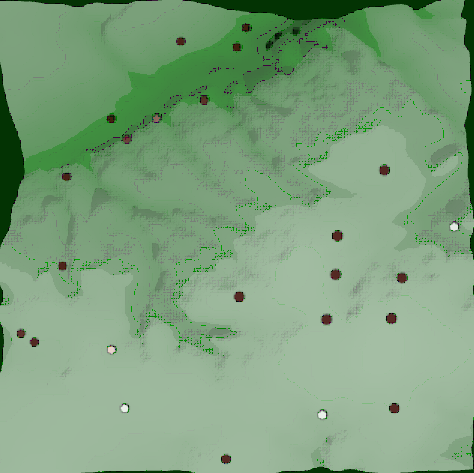
\includegraphics[width=0.32\linewidth]{images/fp1}
                  \-
                  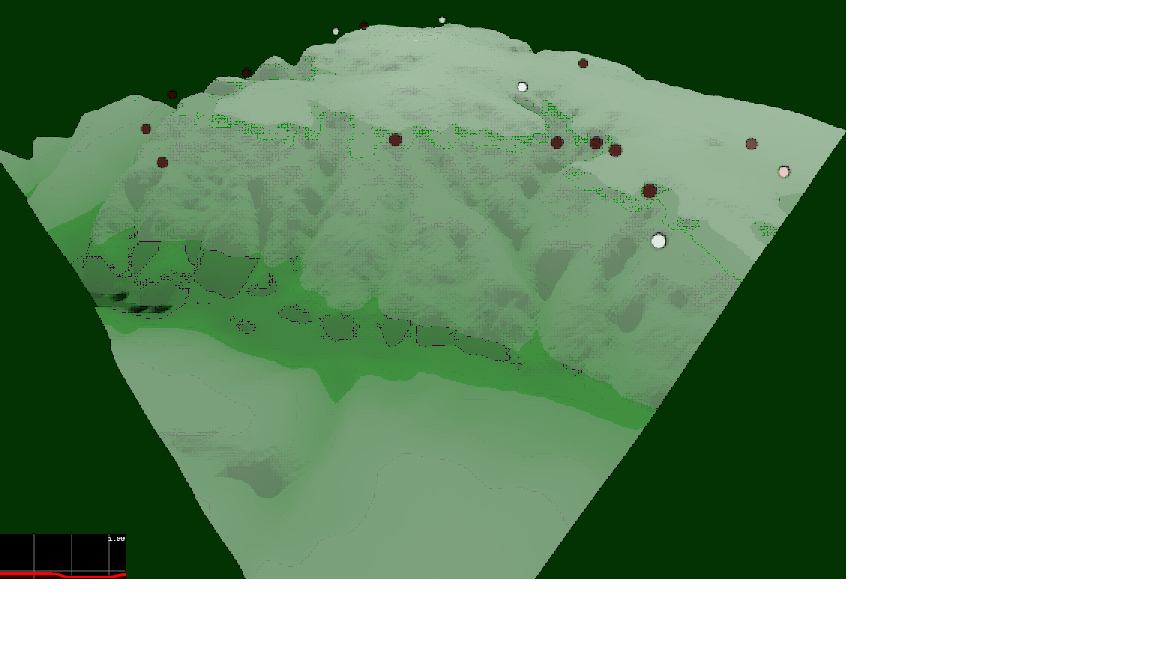
\includegraphics[width=0.32\linewidth]{images/fp2}
                  \-
                  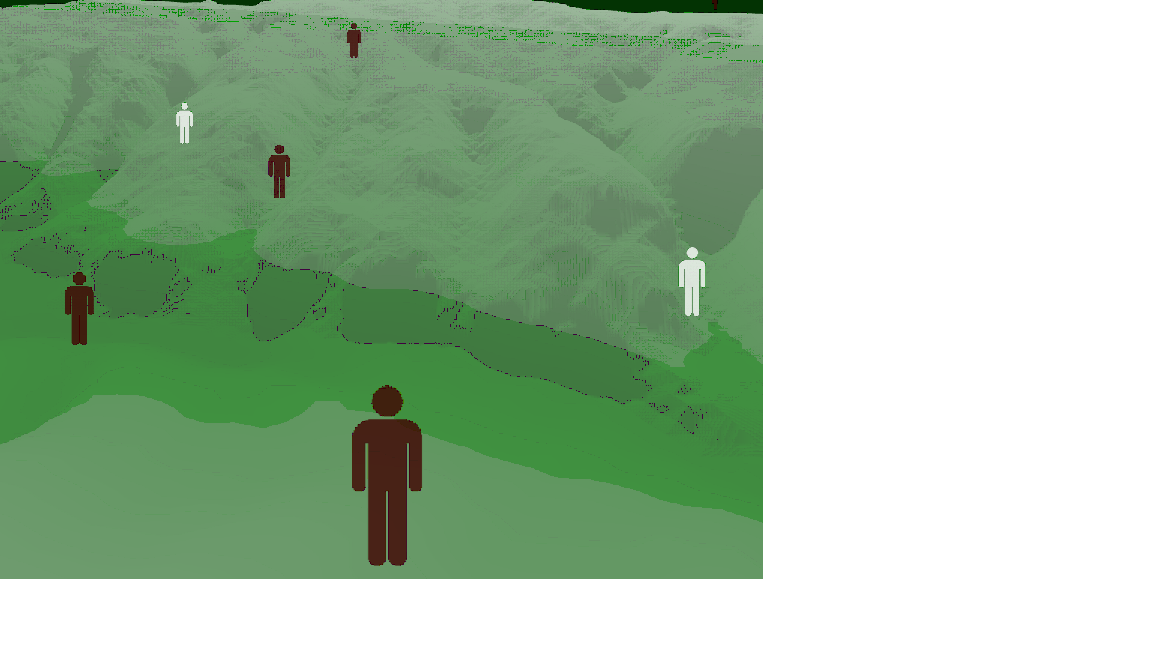
\includegraphics[width=0.32\linewidth]{images/fp3}
                \end{column}
              \end{columns}
            \end{block}
          }
          % ---------------------------------------------------------%
          % end the column
        \end{minipage}
      \end{beamercolorbox}
    \end{column}
    % ---------------------------------------------------------%
    % end the column
  \end{columns}
  \vskip1ex
  %\tiny\hfill\textcolor{ta2gray}{Created with \LaTeX \texttt{beamerposter}  \url{http://www-i6.informatik.rwth-aachen.de/~dreuw/latexbeamerposter.php}}
  \tiny\hfill{Created with \LaTeX \texttt{beamerposter}  \url{http://www-i6.informatik.rwth-aachen.de/~dreuw/latexbeamerposter.php} \hskip1em}
\end{frame}
\end{document}


%%%%%%%%%%%%%%%%%%%%%%%%%%%%%%%%%%%%%%%%%%%%%%%%%%%%%%%%%%%%%%%%%%%%%%%%%%%%%%%%%%%%%%%%%%%%%%%%%%%%
%%% Local Variables:
%%% mode: latex
%%% TeX-PDF-mode: t
%%% End:
